%%% Local Variables:
%%% mode: latex
%%% TeX-master: "../index"
%%% End:

% Recommended:
% DLP
% Problem with Man-in-the-Middle
% How to fix it

\subsection*{Agenda}
\begin{enumerate}
\item DLP
\item Diffie-Hellmann
\item Man-in-the-Middle
\item Authenticated Diffie-Hellmann
\end{enumerate}

\subsection{DLP}
%%% Local Variables:
%%% mode: latex
%%% TeX-master: "../index"
%%% End:

Given a prime $p$ and $\alpha, \beta \in \mathbb{Z}_p^*$ find $a \in \mathbb{Z}_{p-1}$

\textbf{Problem:} For $\beta \equiv \alpha^a \mod p$, find $a$

\textbf{Example:} For $5^a \mod 17 = 4$, find $a$ given 5, 17 and 4. Solution is $a = 12$

\textbf{Requirements}
\begin{enumerate}
\item $p$ must be a large prime\\
  Since $a \in \mathbb{Z}_p$ one can just try all possible $a$s

\item $p - 1$ must have at least one large prime factor to make it
  difficult to prime factor

\item Smallest $m$ for which $\alpha^m \equiv 1 \mod p$ must be large,
  e.i. $\alpha$ should have a high order modulus $p$. \\
  If $\alpha^m
  \equiv 1 \mod p$ then $\alpha^m \equiv \alpha^{a \mod m} \mod p$ so
  there are only $m$ values to check.

  \textbf{Proof:} We can write $a = mq + r$ implying that $r = a \mod m$. Then
  \[ \alpha^a \equiv \alpha^{mq + r} \equiv \alpha^r\alpha^{mq} \equiv
  \alpha^r(\alpha^m)^q \equiv \alpha^r\cdot 1 \equiv \alpha^r \equiv
  \alpha^{a \mod m} \mod p\]
\end{enumerate}

\subsection{Diffie-Hellmann Key Agreement}
\begin{figure}[H]
  \begin{centering}
    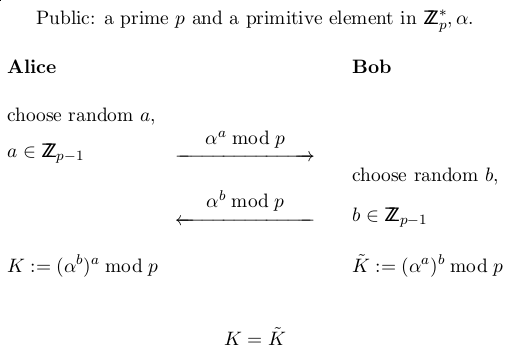
\includegraphics[width=10cm]{images/11-diffie}
    \caption{General model of Diffie-Hellmann Key Agreement}
  \end{centering}
  \label{fig:diffie}
\end{figure}

This keys will now match because exponentiation is commutative:
\begin{align*}
  (\alpha^b)^a &\equiv (\alpha^a)^b \mod p \\
  \alpha^{ab} &\equiv \alpha^{ab} \mod p
\end{align*}

\subsection{Man-in-the-Middle}
Diffie-Hellman is only secure against \emph{passive} adversaries. An
active adversary could simply intercept the transmissions, and switch
the values with her self picked exponents.
\begin{figure}[H]
  \begin{centering}
    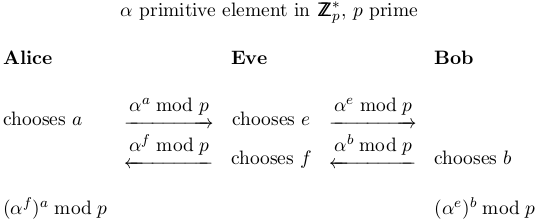
\includegraphics[width=10cm]{images/11-diffie-mitm}
    \caption{Model of Man-in-the-Middle attack on Diffie-Hellmann Key Agreement}
  \end{centering}
  \label{fig:diffie-mitm}
\end{figure}
For Eve to exploit this attack, she has to intercept all transmissions
after the key-agreement has been made, and re-encrypt the messages
because Alice's and Bob's keys \emph{probably} doesn't match.

\subsection{Authenticated Diffie-Hellman}
To prevent MITM attacks, one can use public-key authentication. This
requires that Alice and Bob have each others (certified) public-keys.
\begin{figure}[H]
  \begin{centering}
    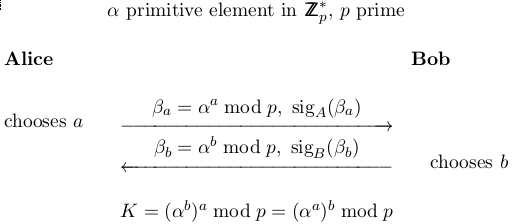
\includegraphics[width=10cm]{images/11-auth-diffie}
    \caption{Model of Authenticated Diffie-Hellman Key Agreement}
  \end{centering}
  \label{fig:auth-diffie}
\end{figure}

The key can now be authenticated with:
\begin{align*}
  K &= (\alpha^b)^a \mod p \\
  \textbf{iff.:}& \\
  \beta_b &= ver_{B_{pub}}(sig_B(\beta_b))
\end{align*}